
%%******************************************************************************
%% SECTION - Viagens Realizadas 
%%******************************************************************************
\setcounter{secnumdepth}{3}
\section{Viagens}
\label{viagens}

A viagem a Usina Jirau aconteceu entre os dias 10 e 13 de Novembro de 2013. A
equipe foi formada por Patrick Paranhos, Ramon Romankeviciuz, Alessandro Jacoud
e Julia Campana. A viagem teve um caráter inicial, o objetivo foi realizar a
reunião de abertura, passando por  uma análise inicial do problema, assim como a
análise de uma operação de Stoplog. Complementarmente, a visita proporcionou ao
grupo a oportunidade de conhecer pessoalmente os responsáveis pelo projeto na
ESBR.
Na reunião de abertura, esclarecemos questões de ordem técnica e também questões
ligadas aos procedimentos da ESBR em Projetos de Pesquisa e Desenvolvimento -
(P$\&$D), assim como foi realizada a assinatura da Ordem de Serviço do Projeto.  Por parte da ESBR estavam presentes Breno Mollinati, Ramon Campos e
Gizele Ferreira. Após a reunião de abertura fomos conduzidos a um pequeno "tour"
pela usina afim de conhecer melhor as instalações e as atividades lá realizadas.

\begin{figure}[ht!]
    \centering 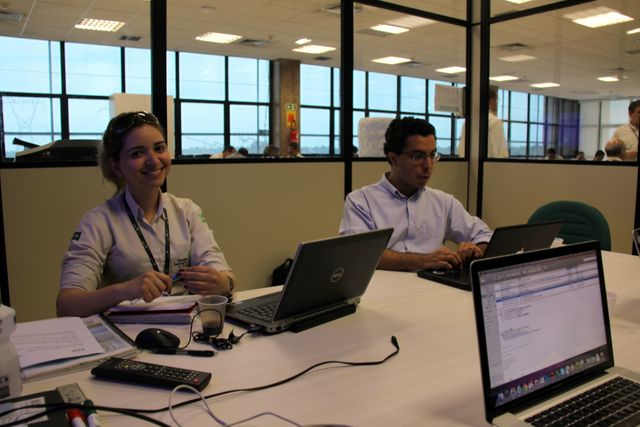
\includegraphics[width=0.6\columnwidth]{figs/jirau/jirau_01}
    \caption{Reunião de abertura.}
    \label{fig:jirau1}
\end{figure}

